\section{Tutela Overview} \label{sec:tutela}

Tutela\footnote{At the time of publication, Tutela is hosted at \url{https://www.tutela.xyz}.}, latin for protection, is a web application that informs users which of their Ethereum addresses are affiliated. Users can search an address, and receive a summary of their anonymity.

\begin{figure}[h!]
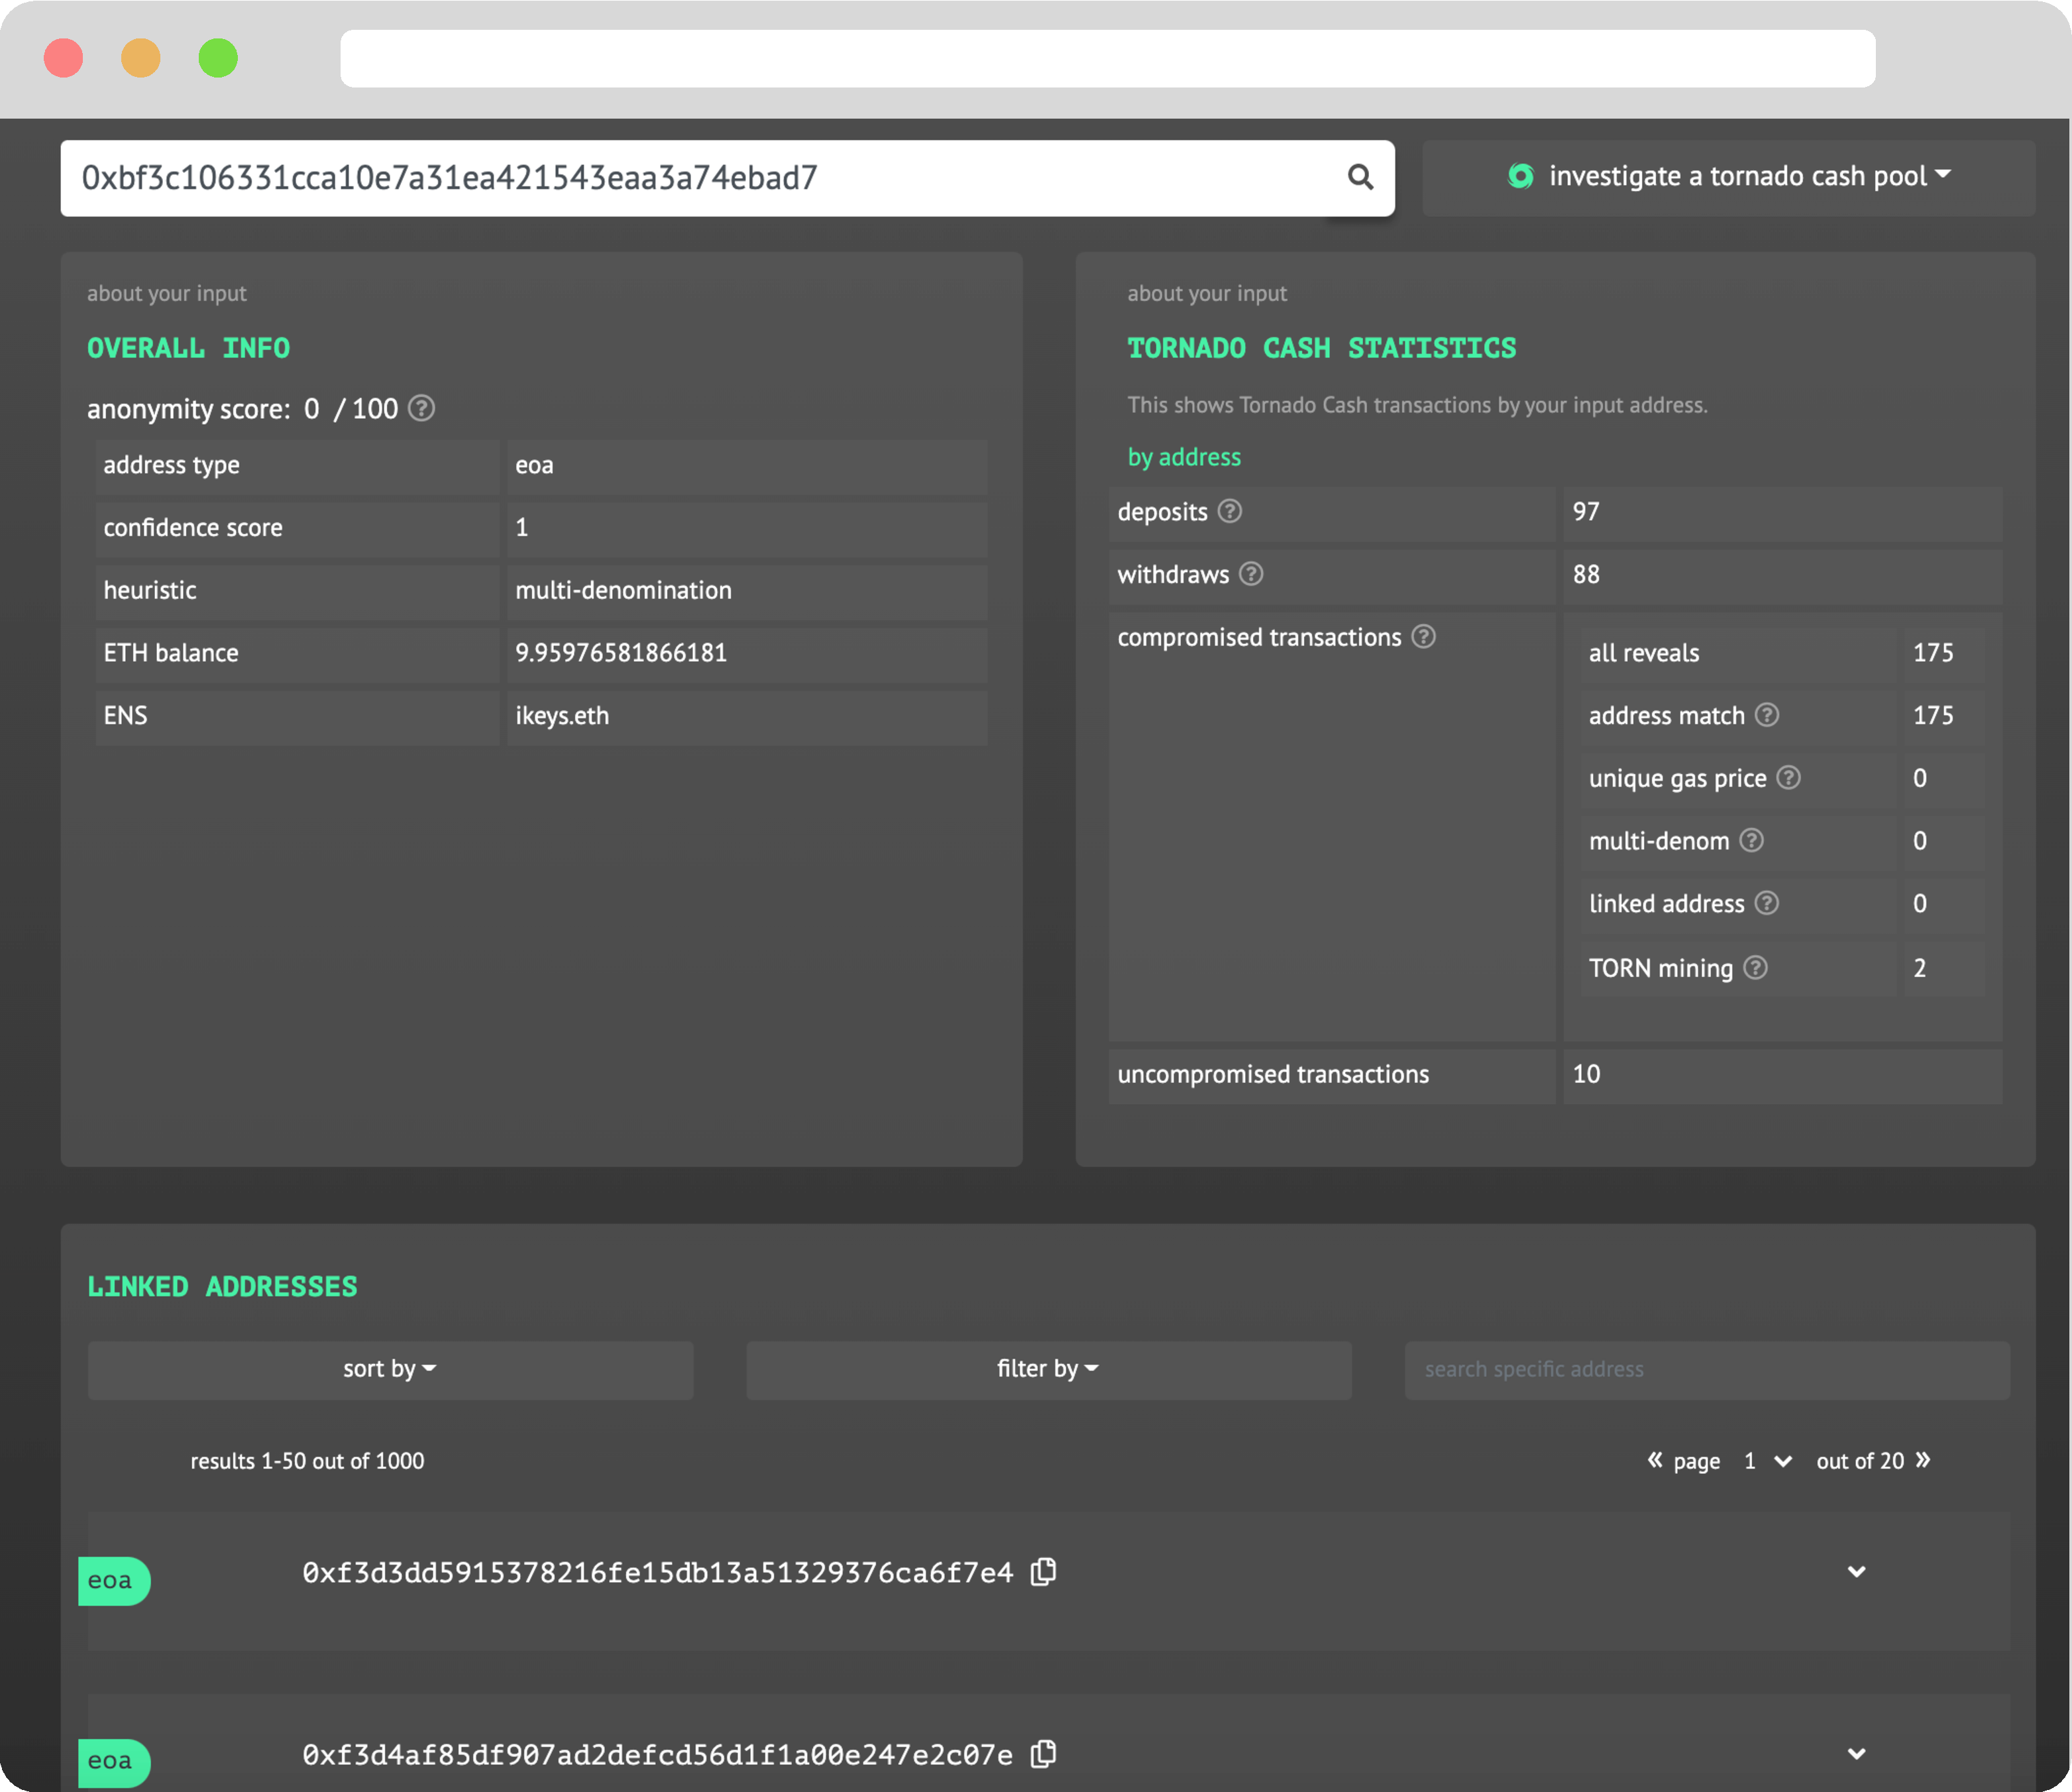
\includegraphics[width=\linewidth]{figures/demo.pdf}
\caption{Tutela interface when searching an Ethereum address. This address is also a Tornado Cash user.}
% \istvan{This figure is too small, I'm afraid.}
% \mike{is this better?}
\label{fig:demo}
\end{figure}

We summarize the main functionalities shown in Figure~\ref{fig:demo}. The response page is separated into three sections. The top left section summarizes the anonymity of the searched address. It contains an ``anonymity score'' out of 100, where a lower number represents less anonymity. In this example, the searched address has an anonymity score of 0, representing a large amount of leaked identity information. Other information, such as balance in ETH or ENS names, are shown when relevant.

The top right section is only populated if the searched address is a Tornado Cash user. In this example, the searched address has deposited 97 times to a Tornado Cash pool while having withdrawn 88 times. Interestingly, we find that through heuristics, we are able to tie 87 of those withdraw transactions to deposit transactions, thereby meaningfully reducing the useful size of the Tornado Cash pool. See Section~\ref{sec:tornado} for more details.

Finally, the bottom section labeled ``Linked Addresses'' shows a list of addresses clustered with the searched one. Each item in this list is denoted as either an externally owned address (EOA), a deposit address, or an exchange address. Each item also contains a confidence score denoting the strength of association with the searched address, and the heuristic that bound it to the searched address.
This example shows a thousand clustered addresses representing an entity with a large wallet portfolio (e.g., bot) -- hence why the anonymity score is zero.

\begin{figure}[h!]
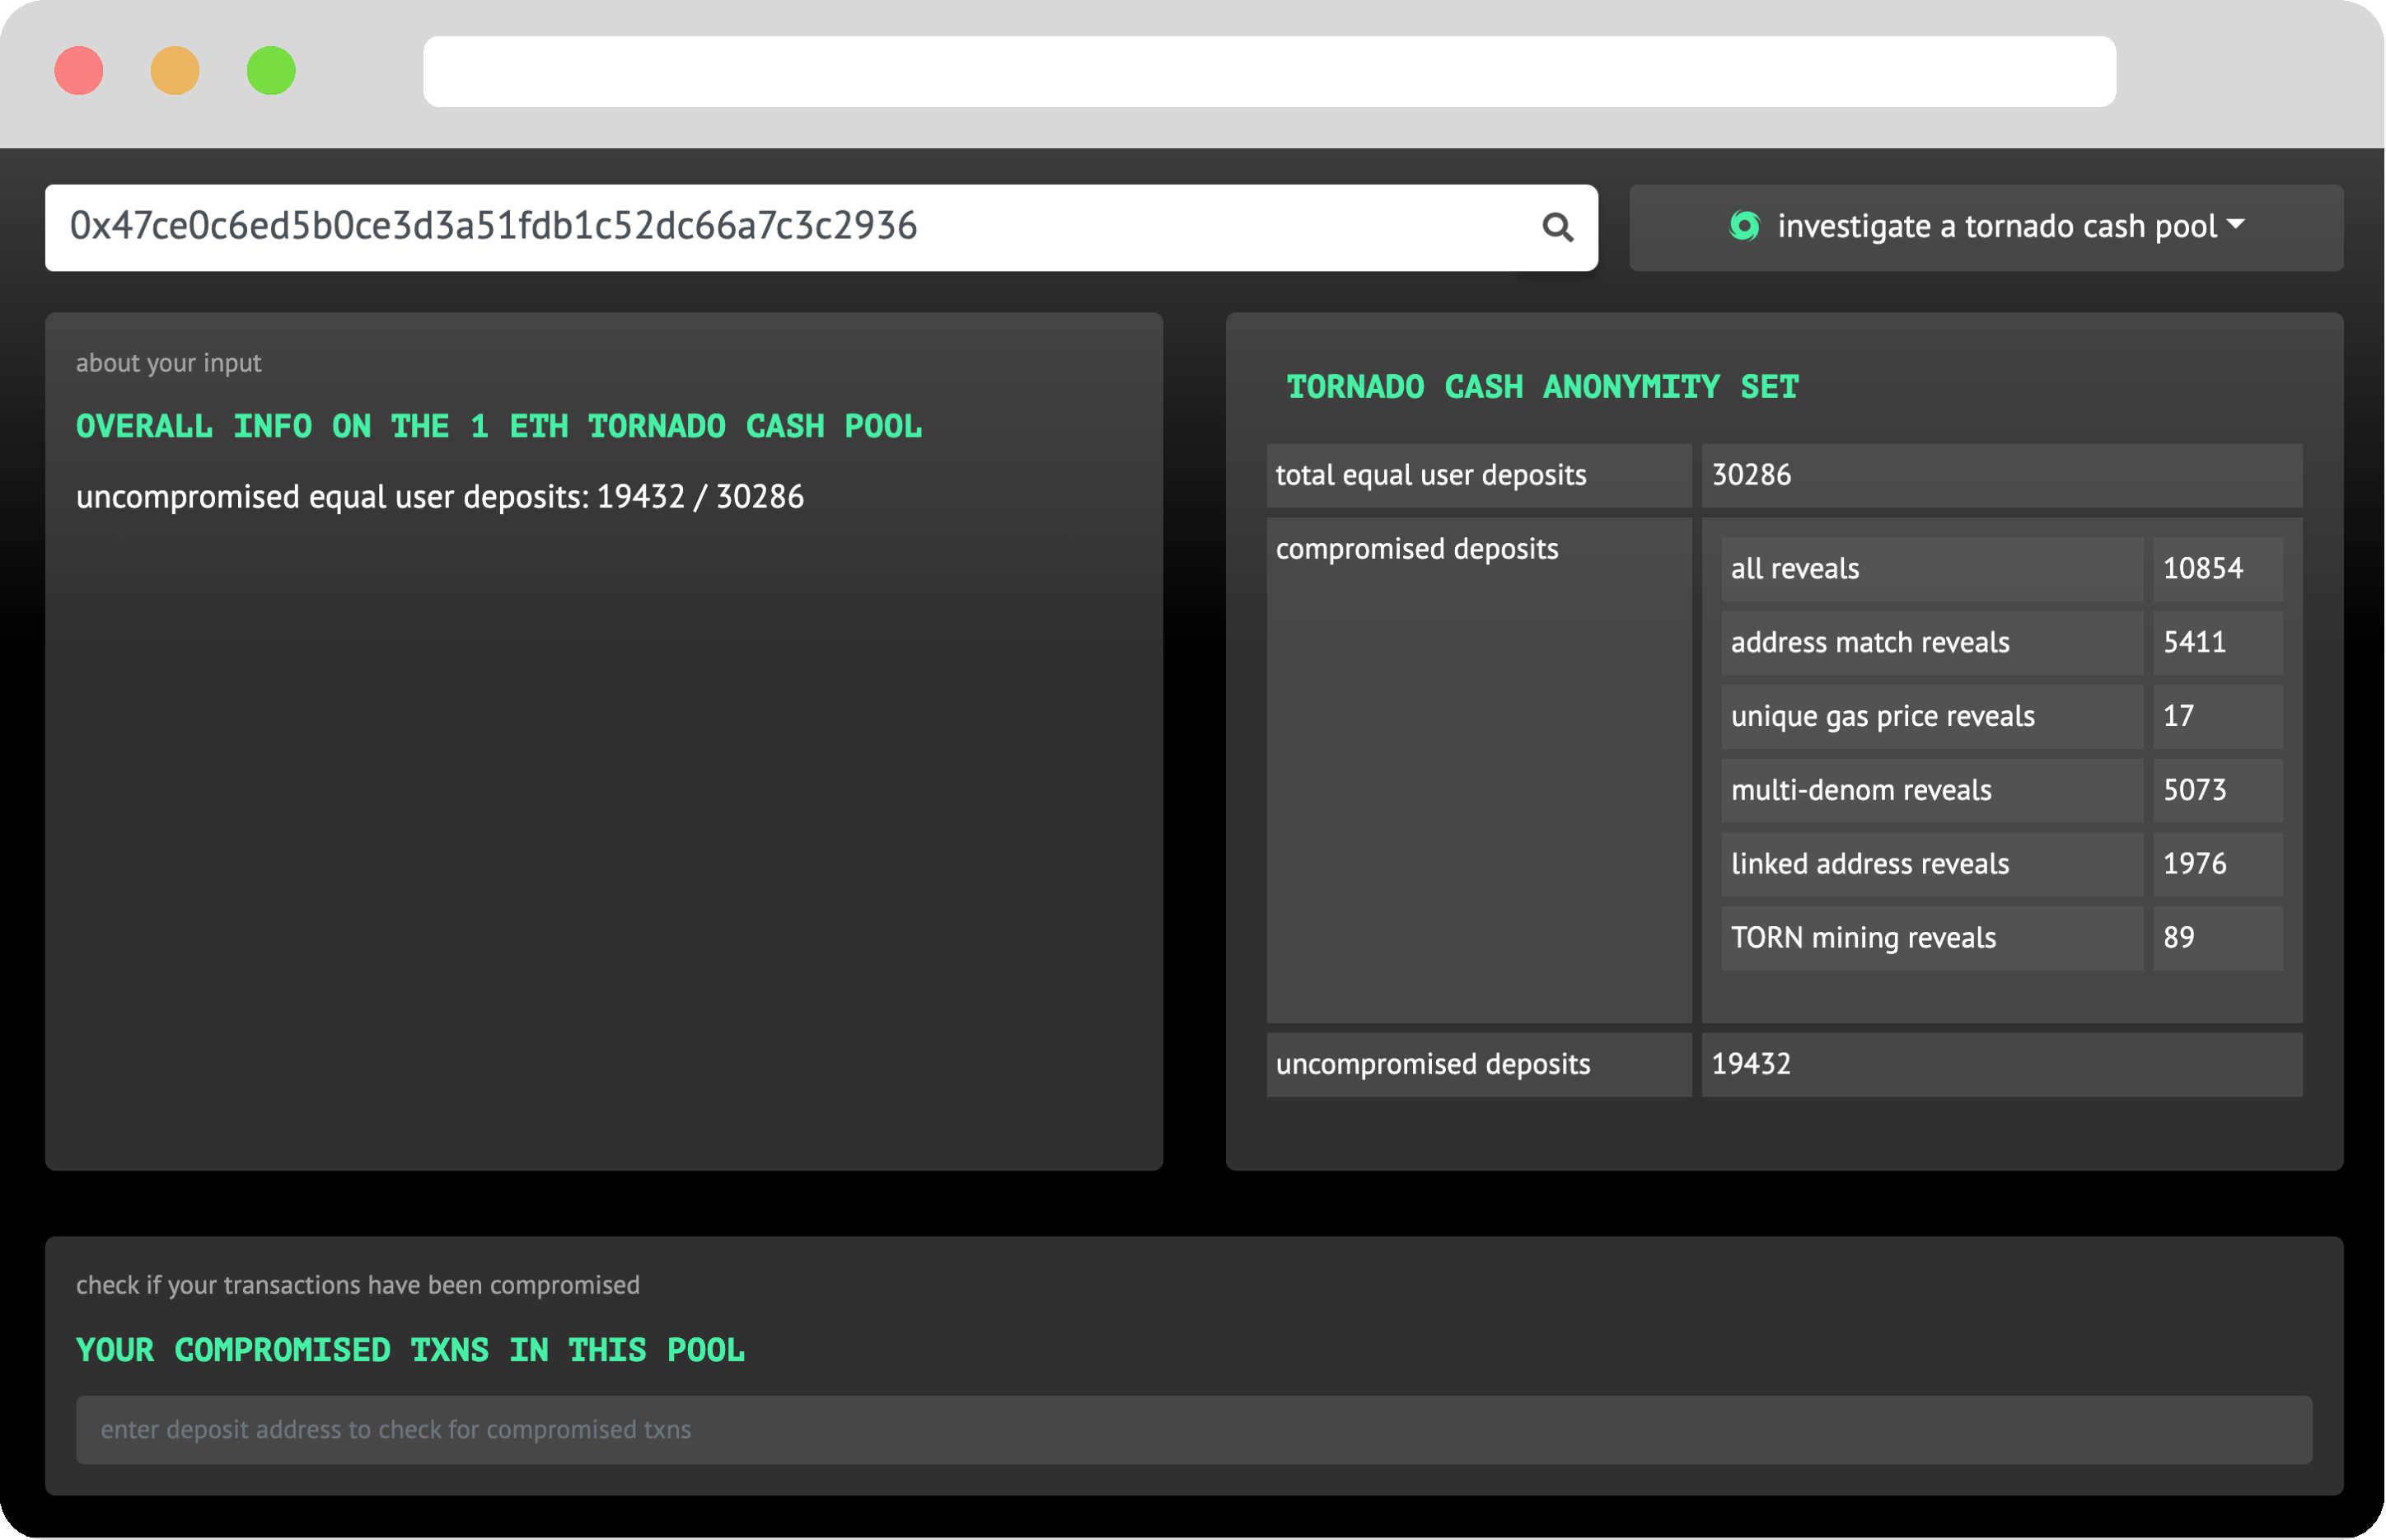
\includegraphics[width=\linewidth]{figures/demo2.pdf}
\caption{Tutela interface when searching an address corresponding to a Tornado Cash pool.}
% \istvan{Too small, maybe?} 
% \mike{is this better?}
\label{fig:demo2}
\end{figure}

If the user searches an address corresponding to a Tornado Cash pool, Tutela has different functionality, shown in Figure~\ref{fig:demo2}. Tornado Cash defines the anonymity set size of each of its pools as the number of equal user deposits. We compute the ``true'' anonymity set size for the pool, subtracting out all equal user deposits that may have been compromised through our heuristics. At the time of publication, the Tornado Cash website reports only the full anonymity set size, not taking into account potential compromises. A concrete use case of Tutela is to adjust this number to protect the privacy of Tornado Cash users more faithfully. 

Lastly, at the bottom of Figure~\ref{fig:demo2}, users can supply an address to check if it has made any compromising transactions in a private way, inspired by the popular website ``Have I been pwned?''\footnote{See \url{https://haveibeenpwned.com}.}.